%%%%%%%%%%%%%%%%%%%%%%%%%%%%%%%%%%%%%%%%%%%%%%%%%%%%%%%%%%%%%%%%%%%%%%
% LaTeX Example: Project Report
%
% Source: http://www.howtotex.com
%
% Feel free to distribute this example, but please keep the referral
% to howtotex.com
% Date: March 2011 
% 
%%%%%%%%%%%%%%%%%%%%%%%%%%%%%%%%%%%%%%%%%%%%%%%%%%%%%%%%%%%%%%%%%%%%%%
% How to use writeLaTeX: 
%
% You edit the source code here on the left, and the preview on the
% right shows you the result within a few seconds.
%
% Bookmark this page and share the URL with your co-authors. They can
% edit at the same time!
%
% You can upload figures, bibliographies, custom classes and
% styles using the files menu.
%
% If you're new to LaTeX, the wikibook is a great place to start:
% http://en.wikibooks.org/wiki/LaTeX
%
%%%%%%%%%%%%%%%%%%%%%%%%%%%%%%%%%%%%%%%%%%%%%%%%%%%%%%%%%%%%%%%%%%%%%%
% Edit the title below to update the display in My Documents
%\title{Project Report}
%
%%% Preamble
\documentclass[paper=a4, fontsize=11pt]{scrartcl}
\usepackage[T1]{fontenc}
\usepackage{fourier}
\usepackage[utf8]{inputenc}
\usepackage{placeins}
\usepackage{makeidx}

\usepackage[portuguese]{babel}	

\usepackage[protrusion=true,expansion=true]{microtype}	
\usepackage{amsmath,amsfonts,amsthm} % Math packages
\usepackage[pdftex]{graphicx}	
\usepackage{url}


%%% Custom sectioning
\usepackage{sectsty}
\allsectionsfont{ \normalfont\scshape}  %% \centering


%%% Custom headers/footers (fancyhdr package)
\usepackage{fancyhdr}
\pagestyle{fancyplain}
\fancyhead{}		% No page header

\fancyfoot[L]{}											% Empty 
\fancyfoot[C]{}											% Empty
\fancyfoot[R]{\thepage}									% Pagenumbering
\renewcommand{\headrulewidth}{0pt}			% Remove header underlines
\renewcommand{\footrulewidth}{0pt}				% Remove footer underlines
\setlength{\headheight}{13.6pt}


%%% Equation and float numbering
\numberwithin{equation}{section}		% Equationnumbering: section.eq#
\numberwithin{figure}{section}			% Figurenumbering: section.fig#
\numberwithin{table}{section}				% Tablenumbering: section.tab#


%%% Maketitle metadata
\newcommand{\horrule}[1]{\rule{\linewidth}{#1}} 	% Horizontal rule

\title{
		%\vspace{-1in} 	
		\usefont{OT1}{bch}{b}{n}
		\normalfont \normalsize \textsc{Universidade de Évora} \\ [25pt]
		\horrule{0.5pt} \\[0.4cm]
		\huge Relatório Teoria da Informação \\
		\horrule{2pt} \\[0.5cm]
}
\author{
		\normalfont 								\normalsize
        José Pinheiro n.º 27167 \\ 
        \normalsize Daniel Ramos n.º 29423\\[-3pt]		\normalsize
        \date{09/01/2014}
}
\date{}


%%% Begin document
\begin{document}
\maketitle

%% Imagem da Universidade
\begin{figure}[h!]
\centering

\includegraphics[scale=1.5]{ue.png}
\end{figure}
\FloatBarrier

%Página de Indice

\pagebreak
\newpage
\tableofcontents
\pagebreak
\newpage
\listoffigures
\pagebreak

%Seccao de Introdução

\section{Introdução}
\horrule{2pt} 

%%%%%%%%%%%%%%%%%%%%%%%%%%%

%Subseccao Descrição
\subsection{Descrição}
	
    \paragraph{} A compressão de dados tem origem na necessidade de transmissão de quantidades maiores de ficheiros e de economização de espaço, exemplo disso são os discos externos, como tal são usados algoritmos de compressão os quais têm como principal objectivo retirar a redundância.
    
    Existem diferentes metodos de compressão
    \begin{itemize}
 	 \item \textbf{Método estatistico:} Este método é usado por vários algorítmos, como por exemplo o algorítmo de Huffman que é um algorítmo de codificação de entropia com código variável sem perdas de informação  que usando matrizes de probabilidades de ocorrência de simbolos e agrupando os mesmos, reduz o número de bits usados para a codificação de uma certa quantidade de informação.
  	 \item \textbf{Método dicionários:} Este outro método é usando por uma diferente categoria de algorítmos. Um exemplo disso são os algorítmos LZW, LZ77 e LZ78, em que a sua capacidade para comprimir dados tem como base a criação de dicionários.
     A medida que um dado ficheiro é lido, se a sequência de caracteres não estiver no dicionário é introduzida e é lhe atribuida uma codificação.
  	\end{itemize}
    \paragraph{} Além dos métodos de compressão, também é necessário analisar os meios de comunicação por onde passam os dados. Esses dados ao serem transmitidos por um canal físico, estão sujeitos a rúido, o que provacam erros aleatórios na recepção dos dados. É aqui que entra o conceito de capacidade de canal, em que um canal recebe um input e produz um output baseado numa distribuição de probabilidade. Para determinar a capacidade de um canal é abordado neste trabalho canais discretos sem memória, que serão calculados usando o algorítmo de R. Blahut.
    
%%%%%%%%%%%%%%%%%%%%%%%%%%%%%
    
%Subseccao Objectivo  
\subsection{Objectivo}
  	\paragraph{} É pretendido com este trabalho que se implemente um algorítmo de compressão/descompressão de imagens binárias em formato PBM, em que será feita uma análise em termos de entropia bem como a implementação do calculo da capacidade de um canal discreto sem memória usando o algorítmo de R. Blahut.
  	
\subsubsection{Compressão}\paragraph{} Nesta parte deste trabalho é pedido que usando uma das linguagens propostas, se crie um algorítmo que comprima imagens no formato descrito anteriormente.
\subsubsection{Descompressão}Deverá ser possível também descomprimir o ficheiro gerado pelo algorítmo de compressão implementado, recuperando a imagem original.
\subsubsection{Entropia}Será necessário também analisar a entropia do ficheiro original, incluíndo a informação mútua. 

\pagebreak
    
 
%%%%%%%%%%%%%%%%%%%%%%%%%%%%%
% Pagina Descriçao

\section{Desenvolvimento}
\horrule{2pt} 
\subsection{Implementação}

\subsubsection{Implementação da compressão de dados e cálculo da Entropia}

%%%%%%%%%%%%%%%%%%%%%%%
%% Arvore de Huffman %%
%%%%%%%%%%%%%%%%%%%%%%%

\paragraph{} Para a realização deste trabalho foi necessário escolher um algorítmo de compressão tendo em conta os algorítmos estudados nas aulas. O escolhido foi o algorítmo de Huffman. A escolha do mesmo teve como principal aspecto a geração de códigos ótimos e uma boa taxa de compressão. Obviamente que o algorítmo de huffman só consegue produzir códigos códigos ótimos se as probabilidades forem potências negativas de base 2.

\paragraph{} De seguida é explicado como foi implementado o processo de compressão/descompressão implementado no trabalho de forma geral. Para mais pormenores, consultar as descrições dos métodos implementados.


\paragraph{Fluxo até chegar a compressão}

\begin{figure}[h!]
\centering
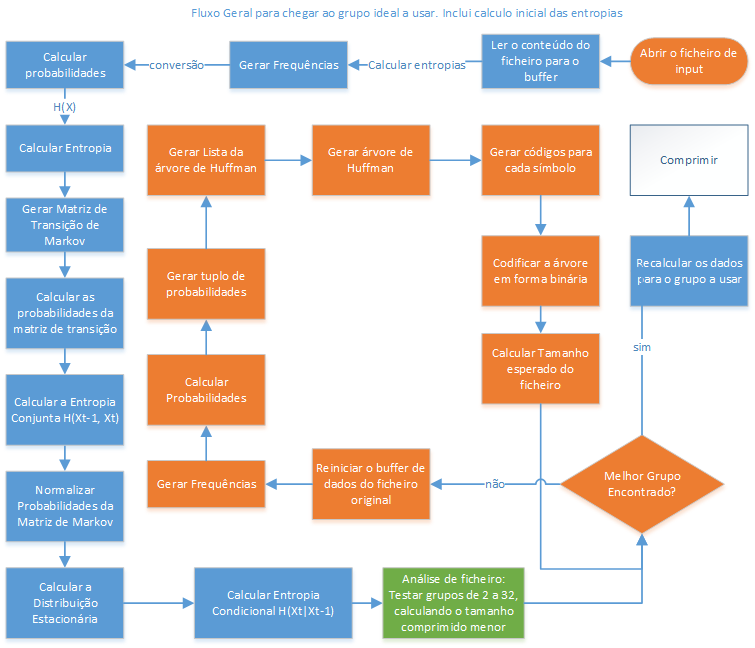
\includegraphics[scale=0.8]{fluxogeral.png} %% {IMAGEM.FORMT}
\caption{\label{fig:fluxogeral}Fluxo geral do compressor até chegar à compressão}
\end{figure}
\FloatBarrier
\paragraph{}
Dado o ficheiro de input, o compressor irá ler o conteúdo do ficheiro para um buffer local para que não seja necessário fazer vários varrimentos ao ficheiro a partir do disco rígido.
\\
De seguida irá ser calculada a entropia, entropia condicional, entropia conjunta e informação mútua. As entropias baseiam-se nas seguintes fórmulas abaixo descritas.
	\begin{align}
  		H(X) &= -\sum p(x) log_{2} p(x)
  	\end{align}
    
    \begin{align}
  	H(xt|xt-1) &= -\sum p(xt-1)\sum p(xt|xt-1) log_{2} p(xt|xt-1)
	\end{align}
    
    \begin{align}
  	H(X,Y) &= -\sum p(x,y) log_{2} p(x,y)
	\end{align}
    
     \begin{align}
  	I(X,Y) &= \sum p(x,y) log_{2} \frac{p(x,y)} {p(x)*p(y)}
	\end{align}
\paragraph{}
Para que seja possível calcular as entropias, é gerado a partir do buffer do ficheiro as frequências que ocorrem para cada símbolo do alfabeto, isto é, zeros e uns. Depois da calculada as frequências, a matriz é transformada em probabilidades, sendo calculada a Entropia H(X) (2.1).
\paragraph{}
Para calcular a entropia condicional e conjunta, é necessário gerar novas matrizes. Neste caso estamos a falar de uma matriz de probabilidade de transição que equivale a uma cadeia de markov, onde é calculada a probabilidade de mudar de estado sabendo o estado anterior.
Começa-se por calcular de novo as frequências de occurrer um símbolo sabendo o símbolo anterior, convertendo as frequências para probabilidades de seguida.
\\
De seguida é calculado a Entropia Conjunta H(x,y) (2.3) sobre a matriz de transição gerada.
\\Para calcular a Entropia condicional é necessário alguns passos adicionais. Começa-se por normalizar as probabilidades, bastando para isso dividir a probabilidade pela soma das probabilidades da coluna correspondente.
O último passo será então calcular a distribuição estacionária que nós dá a distribuição de probabilidades dos estados tal que a distribuição no instante n é igual à distribuição no instante n-1. Com isto é possivel então calcular a entropia H(xt|xt-1) (2.2)
\paragraph{}
Com as entropias calculadas, é fácil cálcular a informação 	mútua, bastanto aplicar a seguinte formula (2.5)
	\begin{align}
  	I(X,Y) &= H(X) - H(X|Y)
	\end{align}

\paragraph{}
Depois de cálculada as entropias, o compressor irá analisar os dados do ficheiro e irá tentar encontrar a melhor taxa de compressão possivel. Para isso é calculado para cada grupo (2 a 32) tendo em conta os seguintes passos:
\begin{itemize}
\item \textbf{Frequências} Cálcula as frequências para o número de bits relativos ao grupo, exemplo: 1111
\item \textbf{Probabilidades} Cálcula as probabilidades baseadas nas frequências
\item \textbf{Tuplo de probabilidades} Gera uma lista de tuplos que contem as probabilidades associadas a cada símbolo.
\item \textbf{Construção da lista para a árvore de huffman}Gerar uma Lista baseado no tuplo de probabilidades para que seja possível gerar uma árvore de Huffman posteriormente. Para que tal seja possivel, a lista é ordenada decrescentemente, sendo retirado os últimos dois tuplos, gerando um novo tuplo com a soma das probabilidades dos dois tuplos removidos. Aqui os tuplos que são compostos por dois símbolos, tem prioridade no sorteamento em relação aos tuplos com apenas um símbolo caso tenham a mesma probabilidade, para que seja possível construir códigos mais curtos.

\item \textbf{Geração da árvore de Huffman}É gerada a árvore de huffman, bastando para isso ler a lista gerada anteriormente, sendo criados nós desde a raiz até aos filhos consoente se existe filhos esquerdos ou direitos na lista.
\item \textbf{Gerarção de códigos por símbolo} É gerado os códigos por cada símbolo na árvore. Os códigos são gerados de forma a que quando se navega na árvore, se ouver filhos às esquerda, é acrescentado um 0 ao código. Se ouver filhos à direita, é acrescentado um 1 ao código.
\item \textbf{Codificação da árvore de Huffman} Neste passo a árvore de Huffman gerada é codificada em binário para que seja escrita no ficheiro comprimido. O processo é bastante simples. É feito um percurso pós-ordem (E, D, N) à árvore, em que é adicionado um 0 se o nó for filho e um 1 se o nó for uma folha, sendo escrito o símbolo em binário de seguida.
Por exemplo 00110010 seria o percurso E E (Folha) (símbolo 1) E E (Folha) (símbolo 0). O número de bits por símbolo está associado ao tamanho do grupo.
\item \textbf{Cálculo do tamanho esperado}Neste último passo é calculado o tamanho esperado do ficheiro comprimido. 
\end{itemize}

Este processo pára quando não for possível reduzir o tamanho do ficheiro para o grupo actual, sendo utilizado o grupo anterior para comprimir os dados.
\pagebreak
\paragraph{Compressão do ficheiro}
\begin{figure}[h!]
\centering
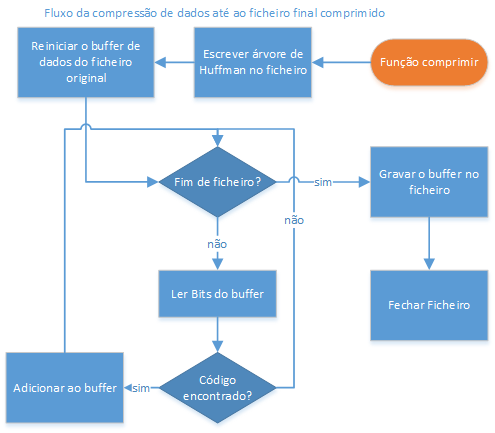
\includegraphics[scale=1]{fluxocompressao.png} %% {IMAGEM.FORMT}
\caption{\label{fig:fluxocompressao}Fluxo da compressão de dados}
\end{figure}
\FloatBarrier
\paragraph{}Calculado o tamanho esperado ao comprimir os dados e o grupo de bits a ser utilizado, será então comprimido o ficheiro.
\\
\paragraph{}Para comprimir os dados será então escrito os dados iniciais correspondentes ao cabeçalho do ficheiro que incluem os seguintes dados:
\begin{itemize}
\item \textbf{Tamanho do ficheiro comprimido} 4 bytes
\item \textbf{Tamanho do grupo} 1 byte
\item \textbf{Tamanho do padding} 1 byte, O padding aqui é o número de zeros que foi acrescentado no fim para conseguir formar o último grupo de bits.
\item \textbf{Codificação da árvore de Huffman} N bits
\end{itemize}
\paragraph{}Escrito os dados do cabeçalho, procede-se então a compressão dos dados originais baseado no grupo de bits calculado.
\\
Será então lidos grupos de bits do buffer que contém os dados do ficheiro através da função Read, que foi implementada para que seja possível ler qualquer grupo de bits escolhido.
Ao ser lido um grupo de bits, é então obtido o seu código através do dicionário de codigos gerados pela árvore de Huffman. Tendo sido validado que existe um código, esse código é então escrito num buffer de output.
\\
Processado o ficheiro na sua totalidade, o buffer é então escrito no ficheiro de destino, concluíndo assim a compressão.

\subsubsection{Implementação da descompressão de dados}
\paragraph{Descompressão do ficheiro}

\begin{figure}[h!]
\centering
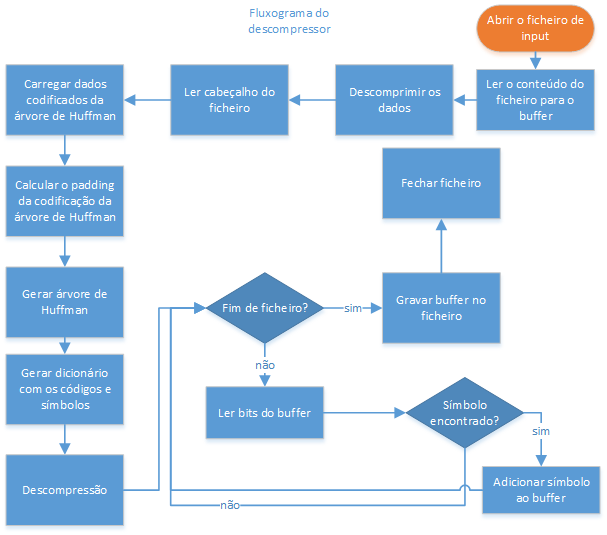
\includegraphics[scale=1]{fluxodescompressao.png} %% {IMAGEM.FORMT}
\caption{\label{fig:fluxodescompressor}Fluxo geral do descompressor}
\end{figure}
\FloatBarrier

\paragraph{}Dado o ficheiro de input, o descompressor irá ler o contúdo do ficheiro para um buffer local para que não seja necessário fazer vários varrimentos ao ficheiro a partir do disco rígido.
\\
De seguida irá ser feito a descompressão do ficheiro, começando por ler o cabeçalho do ficheiro que foi descrito anteriormente. Para que a descompressão seja possível os seguintes passos são efetuados:

\begin{itemize}
  \item \textbf{Carregamento dos dados codificados da árvore de Huffman} Os dados são lidos para uma lista para posterior processamento.
  \item \textbf{Cálculo do padding da codificação da árvore de Huffman} É necessário saber quantos bits extra foram adicionados quando se escreveu os bits correspondentes à codificação da àrvore de Huffman para que a seguinte posição fique alinhada com os dados comprimidos.
  \item \textbf{Criação da árvore de Huffman}Depois de ter sido lida os dados da árvore, é então gerada a árvore de Huffman na sua totalidade que corresponde à árvore original criada, bastando converter os zeros e uns em nós como foi descrito anteriormente na compressão.
  \item \textbf{Geração de códigos->Símbolos}Criada a árvore, é então gerado um dicionário que contem todos os códigos como chave associado a um símbolo.
\end{itemize}
\paragraph{}Criado as condições necessárias para que se possa descomprimir o ficheiro de input, procede-se então a descompressão do ficheiro.
\\
Será então lido um código a partir do buffer em que quando encontrar uma correspondência no dicionário de códigos, o símbolo é então escrito no buffer de output.
Quando o ficheiro de input for lido na sua totalidade, o buffer de output é então escrito no ficheiro de destino na sua forma descomprimida.

\subsubsection{Estructura de dados implementadas}
\paragraph{HuffmanTree}
\paragraph{}Contem métodos que permite criar uma árvore de huffman adaptada ás necessidades do programa desenvolvido. Os seguintes métodos foram implementados, os quais se encontram no ficheiro {\bf HuffmanTree.py}:\\

\begin{itemize}
  \item {\it HuffmanNode:} Incialização do nó da árvore de Huffman, cada nó tem dois filhos, esquerdo e direito.
  
  \item {\it gerarTuploProbabilidades:} Gera tuplos de três elementos (probabilidade, nºaleatorio, simbolo), baseado na matriz de probabilidade recebida. Depois de calculados são inseridos numa lista a ser usada posteriormente para calcular a árvore de Huffman.
  
  \item {\it generateTreeList:} Após receber como argumento uma lista de tuplos de probabilidades e tal como indica, o 1º elemento do tuplo é a probabilidade do símbolo. Também presente neste tuplo, o número aleatório vai diferenciar no caso de haver probabilidades iguais. Este método garante que a árvore contruída é válida.
  
  \item {\it generateTreeList\_:} Esta função chamada pela anterior vai pegar na lista de probabilidades, ordenando e invertendo a ordem dos elementos. São removidos da lista os dois últimos tuplos, sendo estes somados e criado um novo tuplo o qual é adicionado à mesma lista.
  
  \item {\it generateTree:} Recebe a lista gerada anteriormente, chama a função \_\_generateTree\_\_ com o nó inicial da árvore, que corresponde à raiz.
  
  \item {\it \_\_generateTree\_\_:} Ao pegar nos tuplos dentro da lista anteriormente gerada, esta função vai gerar a árvore de Huffman baseado se o elemento à esquerda ou à direita é um tuplo(nós) ou um inteiro (folhas).
  \\
  Caso o elemento for tuplo invoca recursivamente esta função até que restem apenas folhas, a cada chamada recursiva a árvore desce um nível.
  
  \item {\it generateSymbolCodes:} Esta função recebe como argumento a raiz da árvore de Huffman já gerada. Inicializa um dicionário e chama a função \_\_generateSymbolCodes\_\_.
  
  \item {\it \_\_generateSymbolCodes\_\_:} Aqui vai ser gerada a codificação para cada símbolo, em que a função recebe um dicionário, o nó de inicialização, uma posição referente ao índice onde acaba o código do símbolo e uma lista. À medida que vão sendo vistos os nós, é-lhes atribuido um valor que corresponde à direcção que seguiu, ou para a esquerda ou para a direita, 0 e 1 respectivamente. Esse valor é escrito na lista que contem todos os valores lidos até agora. Quando o nó corresponde a uma folha, é então escrito o código correspondente ao símbolo nesse nó, limitado pelo valor da posição actual que corresponde ao indice máxima que é lido da lista.
  
  \item {\it codificarArvore:} Nesta função é codificada a árvore que vai posteriormente ser utilizada para a descompressão. 
  É feito um percurso pós-ordem (E, D, N) à árvore, em que é adicionado um 0 se o nó for filho e um 1 se o nó for uma folha, sendo escrito o símbolo em binário de seguida na lista.
  
  \item {\it writeTreeToFile:} É aqui que a árvore codifiacada é escrita no ficheiro, o primeiro elemento a ser inserido é o tamanho do ficheiro comprimido, seguido do tamanho do grupo, isto é, o número de símbolos a agrupar, o próximo elemento vai ser o padding que é o número de zeros a ser a acrescentado no fim do ficheiro para que seja possivel formar um grupo com os bits restantes do ficheiro original.\\ De seguida é codificada a árvore em formato binário sendo escrito também o seu tamanho no ficheiro. Para finalizar é escrita a árvora codificada no ficheiro com recurso a funções auxiliares da biblioteca NumPy.
  
  \item {\it calcularBitsARemoverNoFim:} Aqui é recebido o tamanho da codificação da árvore e é feito um cálculo de modo a saber quantos bits são precisos remover no fim, correspondente ao padding inserido na compressão. Esta função é usada também noutras funções que não pertencem  à árvore de Huffman.
  
  \item {\it generateTreeFromEncodedList:} Gera uma árvore através de uma lista codificada lida do ficheiro. É inicialmente criada uma pilha de nós, que vai conter os nós que ainda estão por preencher. 
  Cada vez que encontra um zero, verifica se o nó no topo da pilha tem filhos disponiveis por preeencher (esquerda ou direita). Caso aconteça é adicionado um nó a esse filho, sendo adicionado esse filho à pilha.
  Caso seja um 1 encontrado, converte a sequência binária num digito que corresponde ao símbolo, fazendo pop à pilha. 
  \\Quando existirem nós no topo da pilha que tenham ambos os filhos preenchidos faz pop até encontrar um nó com filhos disponiveis.

  \item {\it generateCodesToSymbol:} Gera os simbolos através da árvore de Huffman retornando um dicionário com os códigos e os simbolos correspondentes.
  
  \item {\it \_\_generateCodesToSymbol\_\_:} Percorre a árvore gerada para gerar uma correspondência entre o código e um símbolo. O caminho é feito em pós-ordem em que se for para a esquerda, insere um 0 no código. Se for para a direita, insere um 1. Assim que encontrar um nó que seja folha, o código gerado é inserido no dicionário com o seu símbolo correspondente.
  
\end{itemize}
\pagebreak 			%% quebra de pagina

%%%%%%%%%%%%%%%%%%%%%%%
%%    Compressão     %%
%%%%%%%%%%%%%%%%%%%%%%%
\paragraph{Compressão}
\paragraph{}Contém métodos que permite comprimir um ficheiro. Os seguintes métodos foram implementados, os quais se encontram no ficheiro {\bf Compressor.py}:\\


\begin{itemize}
\item {\it abrirFicheiro:} Abre o ficheiro a comprimir passado no argumento.

\item {\it fecharFicheiro:} Fecha o ficheiro depois de concluir todas as acções sobre o mesmo.

\item {\it lerConteudo:} Lê o conteúdo do ficheiro na sua totalidade para um buffer.
\\Posiciona o handler no fim do ficheiro e calcula o tamanho total do ficheiro.

\item {\it read:}Permite ler N bits de um buffer de dados. O total de bits lido corresponde ao tamanho do grupo. A cada leitura, é usado operações binárias para obter o bit correspondente de um byte específico. Sempre que esse byte é lido na sua totalidade, é lido novamente um novo byte do buffer, sem ignorar o número de bits que faltam ainda por ler para formar um grupo completo.
\\
Caso o buffer tenha sido lido na sua totalidade, é adicionando zeros extra que corresponde ao padding.

\item {\it reiniciarBufferDoFicheiro:} Faz um reset as variaveis de controlo do buffer.

\item {\it calcularEntropia:} Calcula a Entropia para a matriz de probabilidades gerada.

\item {\it calcularProbabilidades:} Calcula uma matriz de probabilidades tendo em conta as frequências com que aparecem os símbolos.

\item {\it calcularProbabilidadesMarkov:} Cálcula as probabilidades tendo como base uma matriz de frequências. Esta matriz corresponde a uma matriz de transição de probabilidades para uma cadeia de Markov \\ Ex:

\begin{center}  
\ M =  \bordermatrix{ 
     	~ & Xt-1 \cr
 	   Xt &0.2 & 0.8 \cr
        ~ &0.8 & 0.2 \cr} 
\end{center}


\item {\it normalizarProbabilidadesMarkov:} Nesta função são normalizadas as probabilidades. Dividindo o valor numa certa posição da matriz pelo somatório da coluna onde está essa probabilidade.

\item {\it MarkovDistEstacionaria:} Calcula a distribuição estacionária com base na matriz de transições calculada previamente.
\item {\it calcularEntropiaCondicional:} Calcula a Entropia Condicional.
\item {\it calcularEntropiaConjunta:} Calcula a Entropia Conjunta. 
\item {\it gerarFrequencias:} Esta função gera as frequências através da leitura do ficheiro analisando as ocorrências de casa símbolo.

\item {\it gerarMatrizFrequenciasMarkov:} Calcula as frequências em relação às transições de um simbolo sabendo o símbolo anterior. Este calculo origina uma matriz de transição de probabilidades de uma cadeia de Markov.

\item {\it comprimir:} Permite comprimir o ficheiro de input, gerando os dados necessários para comprimir o ficheiro com sucesso.

\end{itemize}

\pagebreak 			%% quebra de pagina

%%%%%%%%%%%%%%%%%%%%%%%
%%   Descompressão   %%
%%%%%%%%%%%%%%%%%%%%%%%

\paragraph{Compressão}
\paragraph{}Contém métodos que permite descomprimir um ficheiro. Os seguintes métodos foram implementados, os quais se encontram no ficheiro {\bf Decompressor.py}:\\


\begin{itemize}
\item {\it abrirFicheiro:} Abre o ficheiro a comprimir passado no argumento.
\item {\it lerConteudo:} Lê o conteúdo do ficheiro na sua totalidade para um buffer.
\\Posiciona o handler no fim do ficheiro e calcula o tamanho total do ficheiro.
\item {\it read:}Permite ler N bits de um buffer de dados. O total de bits lido corresponde ao tamanho do grupo. A cada leitura, é usado operações binárias para obter o bit correspondente de um byte específico. Sempre que esse byte é lido na sua totalidade, é lido novamente um novo byte do buffer, sem ignorar o número de bits que faltam ainda por ler para formar um grupo completo.
\item {\it fecharFicheiro:} Fecha o ficheiro depois de concluir todas as acções sobre o mesmo.
\item {\it descomprimir:} permite descomprimir o ficheiro de input, gerando os dados necessários para descomprimir o ficheiro com sucesso.
\end{itemize}
\pagebreak			%% quebra de pagina

%%%%%%%%%%%%%%%%%%%%%%%%%%%%%%%%%%%%%
%%   Capacidade do Canal: Blahut   %%
%%%%%%%%%%%%%%%%%%%%%%%%%%%%%%%%%%%%%

\subsubsection{Capacidade máxima de um Canal}
\paragraph{} A capacidade de um canal é uma teoria criada inicialmente por Shannon e que tem como principal objecto estudar a quantidade de informação fiável que uma determinada fonte emite. Posteriormente esta teoria deu origem a uma outra criada por Blahut e Arimoto mais elegante e simples que a anterior.

\paragraph{}O algorítmo de Blahut permite calcular a capacidade de um canal discreto sem memória em que o cálculo da capacidade é um problema de optimização da informação mútua.
\\
Para o algorítmo em questão, a capacidade do canal pode ser calculada iterativamente até obtermos uma capacidade próxima do valor real.
\paragraph{}  O algoritmo é apresentado no fluxograma seguinte.
%%% Imagem Blahut
\begin{figure}[h!]
\centering
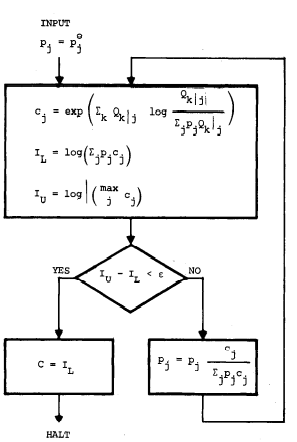
\includegraphics[scale=1.2]{blahut.png}
\end{figure}
\FloatBarrier

\paragraph{} Para calcular a capacidade é necessário uma matriz de distribuição de probabilidade p que corresponde às probabilidades dos símbolos à entrada do canal e uma matriz de transições de probabilidade Q que corresponde a uma cadeia de Markov.
\\
É calculado tambem a capacidade Cj para cada símbolo ao logo das iterações do algorítmo bem como os limite superior e inferior da capacidade calculada.
\\
De seguida faz-se a diferença entre o limite superior e o limite inferior
E calcula-se as capacidades até serem inferiores ao erro escolhido durante a interação.

A capacidade inicial escolhida corresponde ao limite inferior, sendo que se for escolhido o limite superior, a capacidade do canal poderá ficar acima da capacidade real do canal.


\pagebreak 			%% quebra de pagina

%%%%%%%%%%%%%%%%%%%%%%%%%%%%%
% Pagina Conclusão

\section{Conclusão}
\horrule{2pt} 
\subsection{Análise critica de resultados}
\paragraph{} Depois de analisados os resultados obtidos com algumas images. Conseguiu-se obter taxas de compressão para as imagens pequenas de 14\% e taxas de compressão de 89\% para imagens grandes.
\\
Através da entropia conseguimos obter a taxa máxima de compressão para o grupo de bits selecionados e o que se concluíu é que a taxa de compressão real irá sempre ficar abaixo da taxa de compressão máxima devido ao overhead necessário com a inclusão da árvore de huffman, entre outros dados no ficheiro comprimido.
\\
Também se concluíu que para algumas imagens a taxa de compressão dava acima da taxa de compressão máxima, o faz sentido porque o tamanho do ficheiro cresceu, visto que não é possivel sempre comprimir os dados.
\\Para terminar a entropia condicional obtida era sempre menor que a entropia original, o que se faz sentido porque agrupando por sìmbolos, é possivel comprimir mais dados.



%%% End document
\end{document}